%!TEX root = forallxyyc.tex
\part{解释}
\label{ch.semantics}
\addtocontents{toc}{\protect\mbox{}\protect\hrulefill\par}

\chapter{外延性}\label{s:Interpretations}

回想一下，真值函项逻辑是一种真值函项的逻辑。其所有联结词都是真值函项的，并且我们使用真值函项逻辑所能做的\emph{全部}，就是将特定的真值指派给语句。我们可以\emph{直接}做到这一点。例如，我们可以规定真值函项逻辑语句 “$P$” 为真。或者，我们也可以\emph{间接}做到这一点，即提供一个符号化约定，例如：

\begin{ekey}
		\item[P] 大本钟在伦敦。
	\end{ekey}

但是回想一下 \cref{s:TruthFunctionality}，这\emph{仅仅}是指定 “$P$” 真值的一种手段；该符号化约定陈述本质上相当于如下规定：

\begin{itemize}
		\item 真值函项逻辑语句 “$P$” 为真 \ifeff{} 大本钟在伦敦。
	\end{itemize}

并且正如我们在 \cref{s:TruthFunctionality} 中所强调的，真值函项逻辑无法处理那些超越单纯真值差异的意义区别。

\section{符号化与翻译}

一阶逻辑也有其类似的局限。它确实超越了单纯的真值，因为它允许我们将句子拆分为项、谓词和量词。这使得我们可以考虑对于一个特定对象，或是对某些乃至所有对象而言，何者为\emph{真}。\emph{但也就仅此而已}。

具体来说，考虑如下符号化约定：

\begin{ekey}
		\item[\atom{C}{x}] \gap{x} 在卡尔加里教授逻辑 III
	\end{ekey}

这一约定并未将英语谓词的\emph{意义}带入我们的一阶逻辑谓词 “$\atom{C}{x}$” 中。我们只是约定了如下内容：

\begin{itemize}
		\item “$\atom{C}{x}$”与“\gap{x} 在卡尔加里教授逻辑 III”必须\emph{对}完全相同的对象为真。
	\end{itemize}

因此，具体而言：

\begin{itemize}
		\item “$\atom{C}{x}$” 必须对所有（且仅对）在卡尔加里教授逻辑 III 的对象为真（无论这些对象是什么）。
	\end{itemize}

这是\emph{间接}规定谓词对其为真的对象（即其\emph{外延}）的一种方式。

或者，我们也可以\emph{直接}规定谓词的外延。例如，我们可以规定 “$\atom{C}{x}$” 对 Richard Zach，并且仅对 Richard Zach 为真。碰巧的是，这一直接规定与上述间接规定会产生相同的效果，因为只有 Richard Zach 在卡尔加里教授逻辑~III。但重要的是意识到，英语谓词“\blank\ 是 Richard Zach”与“\blank\ 在卡尔加里教授逻辑 III”具有非常不同的含义！

关键在于，一阶逻辑不具备处理意义细微差别的资源。当我们解释一阶逻辑时，我们只关心谓词对哪些对象为真，而无论我们是以直接还是间接的方式来规定这些对象。谓词对其为真的那些对象，称为该谓词的\define{外延}。我们说一阶逻辑是一种\define{外延语言}，因为它不刻画那些具有相同外延的谓词在意义上的差异。

正因如此，我们才称之为将英语句子\emph{符号化}为一阶逻辑。
如果翻译必须保留意义，那么显而易见，我们并非是在将英语\emph{翻译}成一阶逻辑。

\section{外延}\label{sec:extensions}
我们可以直接规定谓词对其为真的对象。而且我们的规定可以随心所欲，甚至颇为任意。例如，我们可以规定 “$\atom{H}{x}$” 应仅对以下对象为真：

\begin{itemize}
		\item 亚里士多德
		\item 数字 $\pi$
		\item 每一台曾制造过的钢琴上的每一个最顶部的 F 键
	\end{itemize}

在采用了对 “$\atom{H}{x}$” 的这一解释之后，假设我们进一步补充符号化约定：

\begin{ekey}
		\item[a] 亚里士多德
		\item[h] 希帕提娅
		\item[p] 数字 $\pi$
	\end{ekey}

那么，在此解释下，“$\atom{H}{a}$” 和 “$\atom{H}{p}$” 都为真，但 “$\atom{H}{h}$” 为假，因为希帕提娅不在我们所规定的对象之列。

这种明确规定的过程，有时被称为规定一个谓词的\emph{外延}。请注意，在我们刚刚给出的规定中，所列对象并无特别的共性。这没有关系。逻辑并不关心我们人类（在某个时刻）认为什么“理所当然属于一类”；对逻辑而言，所有对象都是平等的。

任何定义明确的对象集合，都是一个一元谓词的潜在外延。上面的例子展示了通过\emph{枚举}来规定“$\atom{H}{x}$”之外延的一种方式，即简单地列出“$\atom{H}{x}$”外延中的所有对象。正如我们已经看到的，我们也可以通过给出一个英语谓词来规定外延，例如“\gap{x} 在卡尔加里教逻辑~III”或“\gap{x} 是 $3$ 与 $9$ 之间的偶数”。后者将规定一个由 $4$、$6$ 和 $8$ 组成的外延，且仅包含这三个对象。

注意，一些自然语言谓词，例如“\gap{x} is a round square”（\gap{x} 是一个圆形的方块），不对任何对象为真。此时，我们说该谓词的外延是\emph{空的}。我们确实允许空外延，并且我们可以通过不列出任何成员来简单地规定“$\atom{H}{x}$”的外延为空。（考虑“空无”的集合或许有些奇怪，但逻辑有时就是这么奇怪。）

\section{多元谓词}
对于一元谓词，这一切都相当容易理解，但当我们处理二元谓词时，情况就变得复杂了。考虑如下符号化约定：

\begin{ekey}
		\item[\atom{L}{x,y}] \gap{x} 爱 \gap{y}
	\end{ekey}

依据以上讨论，该符号化约定应被理解为：

\begin{itemize}
		\item “$\atom{L}{x,y}$”与“\gap{x} 爱 \gap{y}”必须对完全相同的对象为真。
	\end{itemize}

因此，特别地：

\begin{itemize}
		\item “$\atom{L}{x,y}$” 应对 x 和 y（按此顺序）为真 \ifeff{} x 爱 y。
	\end{itemize}

这里必须强调顺序，因为爱——众所周知——并非总是相互的。（注意，右边出现的“x”和“y”是\emph{扩展英语}（augmented English）的符号，在此被\emph{使用}。相反，“$\atom{L}{x,y}$”中的“$x$”和“$y$”是一阶逻辑的符号，在此被\emph{提及}。）

这属于间接规定。那么直接规定呢？直接规定也很棘手。如果我们\emph{仅仅}列出属于 “$\atom{L}{x,y}$” 的对象，我们将无法区分哪些是爱者，哪些是被爱者（或二者兼是）。我们必须在明确的规定中包含顺序信息。

为此，我们规定二元谓词对对象的\emph{序对}为真，且序对的顺序至关重要。例如，我们可以规定 “$\atom{B}{x,y}$” 对且仅对以下序对为真：

\begin{itemize}
		\item \ntuple{列宁，马克思}
		\item \ntuple{波伏娃，萨特}
		\item \ntuple{萨特，波伏娃}
	\end{itemize}

这里的尖括号标示了顺序。假设我们现在添加以下规定：

\begin{ekey}
		\item[l] 列宁
		\item[m] 马克思
		\item[b] 波伏娃
		\item[r] 萨特
	\end{ekey}

那么 “$\atom{B}{l,m}$” 为真，因为 \ntuple{列宁，马克思} 在我们的明确列表中；但 “$\atom{B}{m,l}$” 为假，因为 \ntuple{马克思，列宁} 不在列表中。然而，“$\atom{B}{b,r}$” 和 “$\atom{B}{r,b}$” 都为真，因为 \ntuple{波伏娃，萨特} 和 \ntuple{萨特，波伏娃} 都在列表中。

为了使上述观念更严谨，我们需要发展一些非常基础的\emph{集合论}。集合论拥有形式工具来处理外延、有序对等等。然而，本书不涵盖集合论。因此，我将仅以这种非严格的方式呈现这些观念。尽管如此，其核心思想应当是清晰的。

\section{同一性的语义}
同一性是一阶逻辑中一个特殊的谓词。我们书写它的方式与其他二元谓词略有不同：例如写作 “$x=y$” 而非 “$\atom{I}{x,y}$”。但更重要的是，它的解释是唯一且永久固定的。

如果两个名称指称同一个对象，那么互换其中一个名称与另一个，不会改变任何语句的真值。因此，特别地，如果 “$a$” 与 “$b$” 命名了同一个对象，那么以下所有陈述均为真：\label{model.nonidentity}
	\begin{align*}
	 	\atom{A}{a} &\eiff \atom{A}{b} \\
	 	\atom{B}{a} &\eiff \atom{B}{b}\\
		\atom{R}{a,a} &\eiff \atom{R}{b,b}\\
		\atom{R}{a,a} & \eiff \atom{R}{a,b}\\
		\atom{R}{c,a} &\eiff \atom{R}{c,b}\\
		\forall x\, \atom{R}{x,a} &\eiff \forall x\, \atom{R}{x,b}
	\end{align*}
一些哲学家相信这个主张的逆命题。也就是说，他们认为，如果完全相同的语句（不包含 “$=$”）对 x 和 y 为真，那么 x 和 y 就是同一个对象。这是一个极具争议的哲学主张——有时被称为\emph{不可分辨者的同一性}——而我们的逻辑并不采纳它；我们允许完全相同的陈述对两个\emph{不同}的对象为真。

为了阐明这一点，考虑以下解释：

\begin{ekey}
		\item[\text{domain}] P.~D.\ Magnus, Tim Button
		\item[a] P.~D.\ Magnus
		\item[b] Tim Button
		\item[\atom{\metav{R}}{x_1,\dots, x_n}] 对于每个我们在此考虑的原谓词 \metav{R}，该谓词对\emph{任何对象}都不为真。
	\end{ekey}

假设 “$A$” 是一个一元谓词；那么 “$\atom{A}{a}$” 为假且 “$\atom{A}{b}$” 为假，因此 “$\atom{A}{a} \eiff \atom{A}{b}$” 为真。类似地，如果 “$R$” 是一个二元谓词，那么 “$\atom{R}{a,a}$” 为假且 “$\atom{R}{a,b}$” 为假，因此 “$\atom{R}{a,a} \eiff \atom{R}{a,b}$” 为真。依此类推：每一个不涉及 “$=$” 的原子语句都为假，因此每一个连接此类语句的双条件句都为真。尽管如此，Tim Button 和 P.~D.\ Magnus 是两位不同的人，而非同一个人！

\section{解释}
在一阶逻辑中，我们将定义一个\define{解释}，它由以下四部分组成：\footnote{解释也常被称为“模型”或“结构”。}
\begin{compactlist}
    \item 规定一个非空的论域；
    \item 为每个我们考虑的名称，指派论域中恰好一个对象（即该名称的\define{所指}）；
    \item 为每个我们考虑的谓词（除了“$=$”以外）规定该谓词对哪些对象（按何种顺序）为真（即该谓词的\define{外延}）。
\end{compactlist}

对于一元谓词，外延是其为真的那些对象所构成的集合；对于二元谓词，外延是有序对的集合，等等。

我们无需为“$=$”规定任何东西，因为它具有\emph{固定的}意义，即同一性。每个对象只与自身同一。

因此，我们在\cref{ch.FOL}中考虑过的符号化约定，为我们提供了一种非常方便的呈现解释的方式。本章我们将继续使用它们。根据\cref{sec:extensions}的讨论，我们现在也允许通过右边枚举的方式来规定外延，例如：

\begin{ekey}
    \item[\text{domain}] 哲学家, 数字
    \item[\atom{H}{x}] 亚里士多德, 希帕提娅, $\pi$
\end{ekey}

这是一种完全有效的指定解释的方式，如下例也是：
\begin{ekey}
    \item[\text{domain}] $0$, $1$, $2$
    \item[\atom{L}{x,y}] \ntuple{$0$,$1$}, \ntuple{$0$, $2$}, \ntuple{$1$, $2$}
\end{ekey}

我们本可以通过给出英文谓词“\gap{x} is less than \gap{y}”来规定（在这个特定论域上）相同的外延。

\newglossaryentry{interpretation}{
  name = {解释},
  description = {对一个\gls{domain}的规定，以及\glspl{name}所指派的那些对象和\glspl{predicate}对其为真的那些对象}
}

然而，有时\emph{以图表形式}呈现一个解释也很方便。为了（形象地）说明：假设我们只想考虑一个二元谓词“$\atom{R}{x,y}$”。那么我们可以简单地通过在两个对象之间画一个箭头来表示它，并规定“$\atom{R}{x,y}$”对 x 和 y 成立 \ifeff{} 在我们的图表中有一条从 x 指向 y 的箭头。举个例子，我们可以给出：

\begin{center}
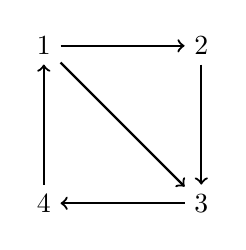
\begin{tikzpicture}
\node (atom1) at (0,2) {$1$};
\node (atom2) at (2,2) {$2$};
\node (atom3) at (2,0) {$3$};
\node (atom4) at (0,0) {$4$};
\draw[->, thick] (atom1)--(atom2);
\draw[->, thick] (atom2)--(atom3);
\draw[->, thick] (atom3)--(atom4);
\draw[->, thick] (atom4)--(atom1);
\draw[->, thick] (atom1) -- (atom3);
\end{tikzpicture}
\bmlDescription{数字 1, 2, 3, 4 由箭头连接。有从 1 指向 2 和 3 的箭头，从 2 指向 3，从 3 指向 4，以及从 4 指向 1 的箭头。}
\end{center}

这个图表可以用来描述一个解释，其论域是前四个正整数，并将“$\atom{R}{x,y}$”解释为仅对以下有序对为真：
\begin{center}
    \ntuple{$1$, $2$},
    \ntuple{$2$, $3$},
    \ntuple{$3$, $4$},
    \ntuple{$4$, $1$},
    \ntuple{$1$, $3$}
\end{center}

同样地，我们也可以给出这个图表：

\begin{center}
\begin{arialabel}{数字 1, 3, 4 由箭头连接。有从 1 指向 3 和自身的箭头，以及从 3 指向 1, 4 和自身的箭头。数字 2 包含在内，但没有箭头进入或指向它。}
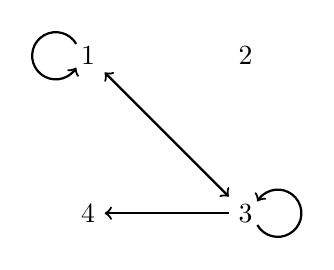
\begin{tikzpicture}
\node (atom1) at (0,2) {$1$};
\node (atom2) at (2,2) {$2$};
\node (atom3) at (2,0) {$3$};
\node (atom4) at (0,0) {$4$};
\draw[->, thick] (atom3)--(atom4);
\draw[->, thick] (atom1)+(-0.15,0.15) arc (-330:-30:.3);
\draw[->, thick] (atom3)+(0.15,-0.15) arc (-150:150:.3);
\draw[<->, thick] (atom1) -- (atom3);
\end{tikzpicture}
\end{arialabel}
\end{center}

由这个图表规定的解释也可以通过列出论域中的元素以及“$\atom{R}{x,y}$”的外延来给出：
\begin{ekey}
    \item[\text{domain}] $1$, $2$, $3$, $4$
    \item[R(x,y)] \ntuple{$1$, $3$},
        \ntuple{$3$, $1$},
        \ntuple{$3$, $4$},
        \ntuple{$1$, $1$},
        \ntuple{$3$, $3$}
\end{ekey}

如果我们愿意，可以让图表更复杂。例如，我们可以添加名称作为特定对象的标签。同样地，为了表示一元谓词的外延，我们可以简单地在某些特定对象周围画一个圈，并规定这些被圈起来的对象（且只有它们）才满足谓词“$\atom{H}{x}$”。为了规定多个谓词，我们可以使用彩色（或虚线、点线）的箭头和圆圈。

\chapter{一阶逻辑中的真}\label{s:TruthFOL}
我们已经介绍了解释。由于解释（除了其他功能外）告诉我们哪些谓词对哪些对象为真，它们将为我们提供原子语句真值的说明。然而，我们现在需要精确地说明，对于一个任意的一阶逻辑语句，在一个解释中为真或为假究竟是什么意思。

我们从\cref{s:FOLSentences}知道，一阶逻辑中有三种类型的语句：
\begin{compactlist}
    \item 原子语句，
    \item 主逻辑算子是语句联结词的语句，
    \item 主逻辑算子是量词的语句。
\end{compactlist}

我们需要为所有这三种类型的语句解释真值。
我们将在本节给出完全一般的解释。不过，为了尽量让解释容易理解，我们会在几个地方使用下面这个解释作为示例：

\begin{ekey}
    \item[\text{domain}] 所有公元2000年以前出生的人
    \item[a] 亚里士多德
    \item[b] 碧昂斯
    \item[\atom{P}{x}] \gap{x} 是哲学家
    \item[\atom{R}{x,y}] \gap{x} 生于 \gap{y} 之前
\end{ekey}

这将是下文\emph{常用的示例}。

\section{原子语句}
原子语句的真值应该是相当直接的。对于语句字母，解释直接规定其为真或为假。语句“$\atom{P}{a}$”为真当且仅当“$\atom{P}{x}$”对“$a$”为真。根据我们的常用示例，这也就是说当且仅当亚里士多德是哲学家。亚里士多德是哲学家，所以该语句为真。同样地，“$\atom{P}{b}$”在我们的常用解释下为假。

类似地，在此解释下，“$\atom{R}{a,b}$”为真当且仅当由“$a$”命名的对象出生于由“$b$”命名的对象之前。亚里士多德确实出生于碧昂斯之前，所以“$\atom{R}{a,b}$”为真。同样地，“$\atom{R}{a,a}$”为假：亚里士多德并非出生于他自己之前。

因此，处理原子语句是非常直观的。当 \metav{R} 是一个 $n$ 元谓词，并且 $\metav{a}_1$、$\metav{a}_{2}$、……、$\metav{a}_{n}$ 是名称时，
\factoidbox{
    语句 $\atom{\metav{R}}{\metav{a}_{1},\metav{a}_{2},\dots,\metav{a}_{n}}$ 在一个解释中为真 \textbf{\ifeff}
    在该解释下，$\metav{R}$ 对由 $\metav{a}_{1}$、$\metav{a}_{2}$、……、$\metav{a}_{n}$（按此顺序）命名的那些对象为真。
}
不过要记住，还有一类特殊的原子语句：由等号连接的两个名称也构成原子语句。这类原子语句同样容易处理。若 \metav{a} 和 \metav{b} 是任意名称，
\factoidbox{
    $\metav{a} = \metav{b}$ 在一个解释中为真 \textbf{\ifeff}
    在该解释下，\metav{a} 和 \metav{b} 命名了完全相同的对象。
}
因此，在我们的常用解释中，“$a = b$”为假，因为亚里士多德和碧昂斯是不同的个体。

\section{句子联结词}
我们在\cref{s:FOLSentences}中看到，一阶逻辑的语句可以用真值函项逻辑中熟悉的真值函项联结词，从更简单的语句构造出来。支配这些真值函项联结词的规则，与我们在真值函项逻辑中所考虑的\emph{完全一样}。它们如下：
\factoidbox{
\begin{factoiditems}
    \item $\metav{A} \eand \metav{B}$ 在一个解释中为真 \textbf{\ifeff} 在该解释下 $\metav{A}$ 与 $\metav{B}$ 均为真。
    \item $\metav{A} \eor \metav{B}$ 在一个解释中为真 \textbf{\ifeff} 在该解释下 $\metav{A}$ 与 $\metav{B}$ 至少有一为真。
    \item $\enot \metav{A}$ 在一个解释中为真 \textbf{\ifeff} 在该解释下 $\metav{A}$ 为假。
    \item $\metav{A} \eif \metav{B}$ 在一个解释中为真 \textbf{\ifeff} 在该解释下 $\metav{A}$ 为假或 $\metav{B}$ 为真。
    \item $\metav{A} \eiff \metav{B}$ 在一个解释中为真 \textbf{\ifeff} 在该解释下 $\metav{A}$ 与 $\metav{B}$ 具有相同的真值。
\end{factoiditems}
}
这与联结词的特征真值表所呈现的信息完全相同，只是呈现方式略有不同。举一些例子或许有助于说明这个想法。（请确保你理解了它们！）在我们的常用解释下：
\begin{itemize}
    \item “$a = a \eand \atom{P}{a}$” 为真。
    \item “$\atom{R}{a,b} \eand \atom{P}{b}$” 为假，因为尽管“$\atom{R}{a,b}$”为真，但“$\atom{P}{b}$”为假。
    \item “$a = b \eor \atom{P}{a}$” 为真。
    \item “$\enot a = b$” 为真。
    \item “$\atom{P}{a} \eand \enot( a= b \eand \atom{R}{a,b})$” 为真，因为“$\atom{P}{a}$”为真而“$a = b$”为假。
\end{itemize}
请确保你理解了这些例子。

\ifHTMLtarget
\section{当主逻辑算子是量词时}
\else
\section[Quantifiers]{当主逻辑算子是量词时}
\fi
\label{s:MainLogicalOperatorQuantifier}

不过，一阶逻辑中令人兴奋的创新在于\emph{量词}的使用，但为量化语句表述真值条件，却比最初想象的更繁琐一些。

这里有一个朴素的最初想法。我们想说“$\forall x\, \atom{F}{x}$”为真当且仅当“$\atom{F}{x}$”对论域中的每一个对象为真。这应该问题不大：我们的解释会直接规定“$\atom{F}{x}$”对哪些对象为真。

不幸的是，这个朴素的想法不够普遍。例如，我们希望能够在（粗略来说）“$\exists y\, \atom{L}{x,y}$” 对论域中每一对象都为真的情况下，断定 “$\forall x \exists y\, \atom{L}{x,y}$” 为真。但我们的解释并\emph{没有直接}规定 “$\exists y\, \atom{L}{x,y}$” 对什么为真。相反，该公式是否对某物为真，应当仅从谓词 “$L$” 的解释、论域以及量词的含义中得出。

因此，我们转向第二个朴素想法。我们可以尝试说，“$\forall x \exists y\, \atom{L}{x,y}$” 在一个解释中为真 \ifeff{} 对我们解释中所包含的\emph{每一个}名称 \metav{a} 而言，$\exists y\, \atom{L}{\metav{a},y}$ 都为真。类似地，我们可以尝试说，$\exists y\, \atom{L}{\metav{a},y}$ 为真当且仅当对我们解释中所包含的\emph{某个}名称 \metav{b} 而言，$\atom{L}{\metav{a},\metav{b}}$ 为真。

不幸的是，这同样不对。为了看清这一点，注意到我们的默认解释只解释了\emph{两个}名称，即 “$a$” 和 “$b$”。但论域（所有公元2000年之前出生的人）所包含的人远多于两个。（而且我们也无意通过命名\emph{所有人}来修正这一点！）

于是我们有了第三种想法。（这次的想法并非朴素，而是正确的。）尽管我们并没有给\emph{每个人}命名，但每个人\emph{都可能}被赋予一个名称。因此，我们应该专注于通过添加一个新名称来扩展解释的可能性。我们将以我们的默认解释为中心，举几个这方面的例子，然后再提出正式定义。

在我们的默认解释中，“$\exists x\, \atom{R}{b,x}$” 应为真。毕竟，在该论域中，确实有人出生在 Beyonc\'e 之后。Lady Gaga 便是其中之一。事实上，如果我们（请注意，这只是临时的）通过添加新名称 “$c$” 来指称 Lady Gaga 以扩展默认解释，那么在此扩展解释上 “$\atom{R}{b,c}$” 将为真。这无疑应足以使得 “$\exists x\, \atom{R}{b,x}$” 在原始默认解释上为真。

在我们的默认解释中，“$\exists x (\atom{P}{x} \eand \atom{R}{x,a})$” 也应为真。毕竟，在该论域中，确实有人既是哲学家又生于亚里士多德之前。苏格拉底就是这样一个人。事实上，如果我们通过让一个新名称 “$c$” 指称苏格拉底来扩展默认解释，那么在此扩展解释上 “$\atom{P}{c} \eand \atom{R}{c,a}$” 将为真。同样，这无疑应足以使得 “$\exists x (\atom{P}{x} \eand \atom{R}{x,a})$” 在原始默认解释上为真。

在我们的默认解释中，“$\forall x \exists y\, \atom{R}{x,y}$” 应为假。毕竟，考虑1999年出生的最后一个人。我们不知道此人是谁，但如果我们通过让一个新名称 “$d$” 指称此人来扩展默认解释，那么我们将无法在论域中找到另一个人并用某个进一步的新名称（例如 “$e$”）去指称，使得 “$\atom{R}{d,e}$” 为真。的确，无论我们用 “$e$” 命名\emph{谁}，“$\atom{R}{d,e}$” 都将为假。这一观察无疑足以使 “$\exists y\, \atom{R}{d,y}$” 在我们扩展的解释中为\emph{假}，而这又无疑足以使 “$\forall x \exists y\, \atom{R}{x,y}$” 在原始默认解释上为假。

如果你理解了这三个例子，那便掌握了要义。这为量化语句的真值定义奠定了基础。

然而，严格来说，我们仍需\emph{给出}那个定义。遗憾的是，结果有些繁琐，且需要引入几个新定义。请做好准备！

假设 \metav{A} 是一个公式。我们将用 $$\metav{A}(\ldots \metav{x} \ldots \metav{x} \ldots)$$ 来表示 \metav{A} 包含若干（通常是一个或多个，但我们也不排除 \metav{x} 根本没有自由出现的情况）变元~\metav{x} 的自由出现。同时假设 \metav{c} 是一个名称。那么，我们将用：
$$\metav{A}(\ldots \metav{c} \ldots \metav{c} \ldots)$$
表示将 \metav{A} 中 $\metav{x}$ 的\emph{每一个}自由出现替换为~$\metav{c}$ 后得到的公式。所得公式称为 $\forall \metav{x}\metav{A}$ 与 $\exists\metav{x}\metav{A}$ 的一个 \define{代入实例}。同时，$\metav{c}$ 被称为 \define{实例化名称}。（如果 \metav{A} 碰巧不含~\metav{x} 的自由出现，则该代入实例就与~\metav{A} 相同。例如，
	$$\exists x (\atom{R}{e,x} \eiff \atom{F}{x})$$
就是
	$$\forall y \exists x (\atom{R}{y,x} \eiff \atom{F}{x})$$
的一个代入实例，其实例化名称是 “$e$”，被实例化的变元是~“$y$”。）

\newglossaryentry{substitution instance}{
  name = 代入实例,
  description = {将一个\gls{formula}中某个\gls{variable}的所有自由出现替换为一个\gls{name}后得到的结果}
}

顺带一提：在用名称替换变元时，我们只允许替换\emph{自由}变元。这是必要的，因为我们允许像 “$\exists x(\forall x\,\atom{F}{x} \eif
\atom{G}{x})$' 这样的公式，其中不同的量词可以约束相同的变元。我们仅将 “$\forall x\,\atom{F}{x} \eif \atom{G}{e}$” 视作该公式的代入实例，而不将 “$\atom{F}{e} \eif
\atom{G}{e}$' 视作代入实例，因为 “$\atom{F}{x}$” 中的 “$x$” 并非自由变元——它被 “$\forall x$” 所约束。（关于这一点，你可能需要回顾 \cref{s:FreeVars}。）

我们的解释会规定哪些名称对应论域中的哪些对象。取论域中任意对象，记为 d，并取一个解释尚未指派的名称 $\metav{c}$。如果我们的解释是 $\mathbf{I}$，则可考虑解释 $\mathbf{I}[\text{d}/\metav{c}]$，它与 $\mathbf{I}$ 完全相同，只是\emph{额外}将对象~d 指派给名称 $\metav{c}$。那么，我们便可以说，对象 d 在解释~$\mathbf{I}$ 下 \define{满足} 公式 $\metav{A}(\dots\metav{x}\dots\metav{x}\dots)$，当且仅当 $\metav{A}(\dots\metav{c}\dots\metav{c}\dots)$ 在 $\mathbf{I}[\text{d}/\metav{c}]$ 下为真。（我们假设名称 $\metav{c}$ 尚未在 $\metav{A}(\dots\metav{x}\dots\metav{x}\dots)$ 中出现。）若 d 满足 $\metav{A}(\dots\metav{x}\dots\metav{x}\dots)$，我们也称 $\metav{A}(\dots\metav{x}\dots\metav{x}\dots)$ \emph{对} d 成立。

\factoidbox{

\begin{factoiditems}
		\item 解释 $\mathbf{I}[\text{d}/\metav{c}]$ 与解释 $\mathbf{I}$ 完全相同，只是额外将对象~d 指派给名称 $\metav{c}$。
		\item 对象 d 在解释~$\mathbf{I}$ 下 \define{满足} $\metav{A}(\dots\metav{x}\dots\metav{x}\dots)$，\textbf{\ifeff} $\metav{A}(\dots\metav{c}\dots\metav{c}\dots)$ 在 $\mathbf{I}[\text{d}/\metav{c}]$ 下为真（其中名称 $\metav{c}$ 未在 $\metav{A}(\dots\metav{x}\dots\metav{x}\dots)$ 中出现过）。
	\end{factoiditems}

}

\newglossaryentry{satisfaction}
{
  name=公式的满足,
  description={指论域中的对象 d 与解释~$\mathbf{I}$ 下的 \gls{formula}~$\metav{A}(\metav{x})$ 之间的一种关系，该关系成立 \ifeff{} $\metav{A}(\metav{c})$ 在修改后的解释 $\mathbf{I}[\text{d}/\metav{c}]$ 中为真，其中 $\metav{c}$ 命名了~d}
}

例如，苏格拉底满足公式~$\atom{P}{x}$，因为 $\atom{P}{c}$ 在解释 $\mathbf{I}[\text{Socrates}/c]$ 下为真，即下面的解释：

\begin{ekey}
	\item[\text{domain}] 所有公元2000年以前出生的人
	\item[a] 亚里士多德
	\item[b] 碧昂丝
	\item[c] 苏格拉底
	\item[\atom{P}{x}] \gap{x} 是哲学家
	\item[\atom{R}{x,y}] \gap{x} 出生在 \gap{y} 之前
\end{ekey}

借助这一记法，大致思路如下。句子 $\forall \metav{x}\metav{A}(\ldots \metav{x} \ldots \metav{x} \ldots)$ 在 $\mathbf{I}$ 下为真 \ifeff{} 对于论域中的每个对象~d，$\metav{A}(\ldots \metav{c} \ldots \metav{c}\ldots)$ 在 $\mathbf{I}[\text{d}/\metav{c}]$ 下为真，即，无论我们用新名称~$\metav{c}$ 来指称论域中的哪个对象。换句话说，$\forall \metav{x} \metav{A}(\ldots \metav{x} \ldots \metav{x}
\ldots)$ 为真 \ifeff{} 论域中每个对象都满足 $\metav{A}(\ldots \metav{x} \ldots \metav{x} \ldots)$。类似地，句子 $\exists \metav{x}\metav{A}(\ldots \metav{x} \ldots \metav{x}
\ldots)$ 在 $\mathbf{I}$ 下为真 \ifeff{} 存在\emph{某个}对象满足 $\metav{A}(\ldots \metav{x} \ldots \metav{x}
\ldots)$，即，对于某个对象~d 和某个新名称~$\metav{c}$，$\metav{A}(\ldots \metav{c} \ldots \metav{c} \ldots)$ 在 $\mathbf{I}[\text{d}/\metav{c}]$ 下为真。
\factoidbox{

\begin{factoiditems}
		\item $\forall \metav{x}\metav{A}(\ldots \metav{x}\ldots\metav{x}\ldots)$ 在一个解释下为真 \textbf{\ifeff} 论域中每个对象都满足 $\metav{A}(\ldots
		\metav{x} \ldots \metav{x}\ldots)$。
		\item $\exists \metav{x}\metav{A}(\ldots \metav{x}\ldots\metav{x}\ldots)$ 在一个解释下为真 \textbf{\ifeff} 论域中至少有一个对象满足 $\metav{A}(\ldots \metav{x}\ldots\metav{x}\ldots)$。
		\end{factoiditems}

	}
需要明确的是：所有这些工作只是（以一种非常迂腐的方式）将上面阐述的直观想法形式化。结果有些繁琐，最终的定义可能略显晦涩。但希望其\emph{核心思想}是清晰的。

\practiceproblems
\solutions
\problempart
\label{pr.TorF1}
考虑以下解释：

\begin{itemize}
		\item 论域仅包含 Corwin 和 Benedict
		\item “$\atom{A}{x}$” 对 Corwin 和 Benedict 都为真
		\item “$\atom{B}{x}$” 仅对 Benedict 为真
		\item “$\atom{N}{x}$” 不对任何人为真
		\item “$c$” 指称 Corwin
	\end{itemize}

判断以下每个句子在该解释下是真还是假：

\begin{compactlist}
\item $\atom{B}{c} $
\item $\atom{A}{c}  \eiff \enot \atom{N}{c}$
\item $\atom{N}{c}  \eif (\atom{A}{c} \eor \atom{B}{c})$
\item $\forall x\, \atom{A}{x}$
\item $\forall x \enot \atom{B}{x}$
\item $\exists x(\atom{A}{x} \eand \atom{B}{x})$
\item $\exists x(\atom{A}{x} \eif \atom{N}{x})$
\item $\forall x(\atom{N}{x} \eor \enot \atom{N}{x})$
\item $\exists x\, \atom{B}{x} \eif \forall x\, \atom{A}{x}$
\end{compactlist}

\problempart
\label{pr.TorF2}
考虑以下解释：

\begin{itemize}
		\item 论域仅包含 Lemmy, Courtney 和 Eddy
		\item “$\atom{G}{x}$” 对 Lemmy, Courtney 和 Eddy 都为真。
		\item “$\atom{H}{x}$” 仅对 Courtney 为真
		\item “$\atom{M}{x}$” 仅对 Lemmy 和 Eddy 为真
		\item “$c$” 指称 Courtney
		\item “$e$” 指称 Eddy
	\end{itemize}

判断以下每个句子在该解释下是真还是假：

\begin{compactlist}
\item $\atom{H}{c} $
\item $\atom{H}{e} $
\item $\atom{M}{c}  \eor \atom{M}{e}$
\item $\atom{G}{c}  \eor \enot \atom{G}{c}$
\item $\atom{M}{c}  \eif \atom{G}{c}$
\item $\exists x\, \atom{H}{x}$
\item $\forall x\, \atom{H}{x}$
\item $\exists x\, \enot \atom{M}{x}$
\item $\exists x(\atom{H}{x} \eand \atom{G}{x})$
\item $\exists x(\atom{M}{x} \eand \atom{G}{x})$
\item $\forall x(\atom{H}{x} \eor \atom{M}{x})$
\item $\exists x\, \atom{H}{x} \eand \exists x\, \atom{M}{x}$
\item $\forall x(\atom{H}{x} \eiff \enot \atom{M}{x})$
\item $\exists x\, \atom{G}{x} \eand \exists x \enot \atom{G}{x}$
\item $\forall x\exists y(\atom{G}{x} \eand \atom{H}{y})$
\end{compactlist}

\problempart
\label{pr.TorF3}
遵循在\cref{s:Interpretations}末尾引入的图示惯例，考虑以下解释：


\begin{center}
\begin{arialabel}{数字 1、2、3、4、5 由箭头连接。存在从 1 到 2、3、4、5 以及到自身的箭头，从 2 到 5 的箭头，从 5 到自身的箭头，以及从 4 到 1 的箭头。3 没有箭头射出。}
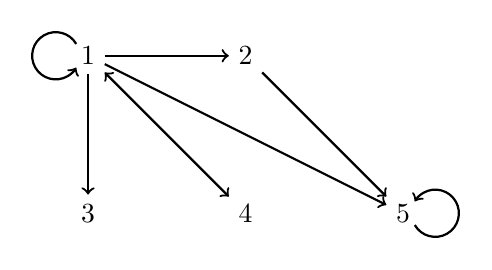
\begin{tikzpicture}
\node (atom1) at (0,2) {$1$};
\node (atom2) at (2,2) {$2$};
\node (atom4) at (0,0) {$3$};
\node (atom5) at (2,0) {$4$};
\node (atom6) at (4,0) {$5$};
\draw[->, thick] (atom1)+(-0.15,0.15) arc (-330:-30:.3);
\draw[->, thick] (atom6)+(0.15,-0.15) arc (-150:150:.3);
\draw[->, thick] (atom1) -- (atom2);
\draw[->, thick] (atom1) -- (atom4);
\draw[<->, thick] (atom1) -- (atom5);
\draw[->, thick] (atom1) -- (atom6);
\draw[->, thick] (atom2) -- (atom6);
\end{tikzpicture}
\end{arialabel}
\end{center}


确定以下每个句子在该解释下是真的还是假的：


\begin{compactlist}
\item $\exists x\, \atom{R}{x,x}$
\item $\forall x\, \atom{R}{x,x}$
\item $\exists x \forall y\, \atom{R}{x,y}$
\item $\exists x \forall y\, \atom{R}{y,x}$
\item $\forall x \forall y \forall z ((\atom{R}{x,y} \eand \atom{R}{y,z}) \eif \atom{R}{x,z})$
\item $\forall x \forall y \forall z ((\atom{R}{x,y} \eand \atom{R}{x,z}) \eif \atom{R}{y,z})$
\item $\exists x \forall y\, \enot \atom{R}{x,y}$
\item $\forall x(\exists y\, \atom{R}{x,y} \eif \exists y\, \atom{R}{y,x})$
\item $\exists x \exists y (\enot x = y \eand \atom{R}{x,y} \eand \atom{R}{y,x})$
\item $\exists x \forall y(\atom{R}{x,y} \eiff x = y)$
\item $\exists x \forall y(\atom{R}{y,x} \eiff x = y)$
\item $\exists x \exists y(\enot x = y \eand \atom{R}{x,y} \eand \forall z(\atom{R}{z,x} \eiff y = z))$
\end{compactlist}

\chapter{语义概念}

\section{有效性、蕴涵等}

在一阶逻辑中定义真相当繁琐。但现在既然已经完成，我们就可以定义其他各种核心逻辑概念。这些定义看起来与真值函项逻辑中的定义非常相似（参见\cref{s:SemanticConcepts}）。然而，请记住这里涉及的是\emph{解释}，而非赋值。

我们将像在真值函项逻辑中那样，在一阶逻辑中也使用符号“$\entails$”。因此，
语句 $\metav{A}_1, \metav{A}_2, \ldots, \metav{A}_n$
\define{蕴涵}语句 $\metav{C}$，
	$$\metav{A}_1, \metav{A}_2, \ldots, \metav{A}_n \entails\metav{C},$$
\ifeff{} 不存在一个解释，在其中所有 $\metav{A}_1$, $\metav{A}_2$, \dots, $\metav{A}_n$ 都为真而 $\metav{C}$ 为假。由此可得，
	$$\entails\metav{A}$$
意味着 $\metav{A}$ 在每一个解释中均为真。

其他逻辑概念在一阶逻辑中也有相应的定义：

\factoidbox{


\begin{factoiditems}
		\item 一个一阶逻辑语句 $\metav{A}$ 是\define{有效式} \ifeff{}
		$\metav{A}$ 在每一个解释中均为真；即 $\entails\metav{A}$。
\newglossaryentry{validity}
{
name=逻辑有效式,
description={一个在每一个\gls{interpretation}下都为真的\gls{sentence of FOL}}
}

		\item $\metav{A}$ 是\define{矛盾式} \ifeff{} $\metav{A}$
		在每一个解释中均为假；即 $\entails\enot\metav{A}$。
\newglossaryentry{contradiction of FOL}
{
  name=矛盾式（一阶逻辑）,
  text=矛盾式,
description={一个在每一个\gls{interpretation}下都为假的\gls{sentence of FOL}}
}

		\item $\metav{A}_1, \metav{A}_2, \ldots, \metav{A}_n \therefore
		\metav{C}$ 是\define{有效的（于一阶逻辑中）} \ifeff{} 不存在一个解释，使得所有前提为真且结论为假；即 $\metav{A}_1,\metav{A}_2,\ldots,
		\metav{A}_n \entails\metav{C}$。否则它是\define{无效的（于一阶逻辑中）}。
\newglossaryentry{valid in FOL}
{
  name=论证的有效性（一阶逻辑）,
  text = 有效,
description={论证所具有的性质；一个论证是有效的当且仅当没有\gls{interpretation}能使所有前提为真而结论为假}
}

		\item 两个一阶逻辑语句 \metav{A} 和 \metav{B} 是\define{等值的} \ifeff{} 它们在完全相同的解释中彼此同为真；即同时有
		$\metav{A}\entails\metav{B}$ 和 $\metav{B}\entails\metav{A}$。

\newglossaryentry{equivalent in FOL}
{
  name=等值性（一阶逻辑）,
  text = 等值,
description={成对的\glspl{sentence of FOL}所具有的性质，当且仅当这些句子在每一个\gls{interpretation}下都有相同的真值}
}

		\item 一阶逻辑语句 $\metav{A}_1$, $\metav{A}_2$, \dots,
		$\metav{A}_n$ 是\define{共同可满足的} \ifeff{} 存在某个解释使它们全部为真。它们是\define{共同不可满足的} \ifeff{} 不存在这样的解释。
\newglossaryentry{satisfiable in FOL}
{
  name=可满足性（一阶逻辑）,
  text=共同可满足,
  description={\glspl{sentence of FOL}所具有的性质，当且仅
  当存在某个\gls{interpretation}能使所有这些句子同时为真}
}
	\end{factoiditems}


}

注意，我们使用“有效式”这一标准术语来指称在每一解释下都为真的句子。有效式之于一阶逻辑，就如同重言式之于真值函项逻辑。

\section{表达力}

在\cref{s:MainLogicalOperatorQuantifier}中引入的“对象满足含一个自由变元的公式”这一概念，也可以扩展到含多个自由变元的公式。如果我们有一个
公式 $\metav{A}(\metav{x},\metav{y})$ 带有两个自由变元 $\metav{x}$ 和 $\metav{y}$，那么我们可以说一个对象对 $\langle a, b\rangle$ 满足 $\metav{A}(\metav{x},\metav{y})$
\ifeff{} $\metav{A}(\metav{c},\metav{d})$ 在通过添加两个名称 $\metav{c}$ 和 $\metav{d}$ 而扩展的解释中为真，其中 $\metav{c}$ 指称~$a$ 而 $\metav{d}$ 指称~$b$。举例来说，$\langle \text{Socrates}, \text{Plato}\rangle$ 满足
$\atom{R}{x,y}$，因为在这个解释中 $\atom{R}{c,d}$ 为真：

\begin{ekey}
	\item[\text{domain}] 公元2000年前出生的所有人
	\item[a] Aristotle
	\item[b] Beyonc\'e
	\item[c] Socrates
	\item[d] Plato
	\item[\atom{P}{x}] \gap{x} 是哲学家
	\item[\atom{R}{x,y}] \gap{x} 出生于 \gap{y} 之前
\end{ekey}

对于原子公式，满足它们的对象、对象对等，正是解释中给出的谓词的外延。但“满足”这一概念也适用于非原子公式，例如，公式 $\atom{P}{x} \land \atom{R}{x,b}$ 被所有在 Beyonc\'e 之前出生的哲学家所满足。它甚至适用于包含量词的公式，例如，$\atom{P}{x} \eand \lnot\exists y(\atom{P}{y} \land \atom{R}{y,x})$ 被所有本身是哲学家且没有别的哲学家出生于他们之前的人所满足——换句话说，该公式对于第一位哲学家为真。

通过考虑带有两个自由变元的公式（可能包含量词），我们可以表达那些在我们的解释或符号化约定中没有专门谓词符号的关系。考虑公式 $\atom{R}{x,y}$。它表达了“\gap{x} 出生于 \gap{y} 之前”这一关系，因为我们正是这样规定其外延的。如果我们交换变元，也就是考虑“$\atom{R}{y,x}$”，会发生什么？论域中的一个对象对 \ntuple{$\text{y}, \text{x}$}（即一对人）满足 $\atom{R}{y,x}$ 当且仅当，反过来的一对 \ntuple{$\text{x}, \text{y}$} 满足 $\atom{R}{x,y}$。换句话说，$\atom{R}{y,x}$ 表达的是“\gap{x} 出生于 \gap{y} \emph{之后}”这一关系。或者假设我们在解释中添加一个表示“……是……的老师”的谓词。


\begin{ekey}
	\item[\atom{T}{x,y}] \gap{x} 是 \gap{y} 的老师
\end{ekey}


那么公式“$\exists z(\atom{T}{z,x} \land \atom{T}{z,y})$”被 x 和 y 满足当且仅当，存在某个人 z 既是 x 的老师也是 y 的老师，也就是说，它表达了“\gap{x} 和 \gap{y} 有共同的老师”。类似地，“$\forall z(\atom{T}{x,z} \eiff \atom{T}{y,
z})$”表达了“\gap{x} 和 \gap{y} 教的是同一批人”。

这些例子的要旨是，有些英语谓词，比如“\gap{x} 和 \gap{y} 有共同的老师”，有时即使没有现成的明确谓词符号，也可以在解释中表达出来。如果是这种情况，你可以使用一个表达该谓词的公式（比如“$\exists
z(\atom{T}{z,x} \land \atom{T}{z,y})$”）来符号化涉及该谓词的英语句子。

\practiceproblems

\problempart
给定以下解释：


\begin{ekey}
	\item[\text{domain}] 所有人
	\item[\atom{W}{x}] \gap{x} 是女性（或女孩）
	\item[\atom{M}{x}] \gap{x} 是男性（或男孩）
	\item[\atom{Y}{x,y}] \gap{x} 比 \gap{y} 年轻
	\item[\atom{O}{x,y}] \gap{x} 是 \gap{y} 的后代
	\item[d] Dana
	\item[a] Alex
\end{ekey}


用公式表达以下关系：


\begin{compactlist}
	\item \gap{x} 比 \gap{y} 年长
	\item \gap{x} 是 \gap{y} 的母亲
	\item \gap{x} 和 \gap{y} 是兄弟姐妹（注意：自己不能是自己的兄弟姐妹）
	\item \gap{x} 是 \gap{y} 的兄弟
\end{compactlist}

\problempart
使用上一练习中的符号化约定，将以下句子符号化：


\begin{compactlist}
	\item Alex 和 Dana 是姐妹。
	\item 父亲都比他们的孩子年长。
	\item Alex 的父母年龄相同。
\end{compactlist}

\chapter{使用解释}
\label{sec.UsingModels}

\section{有效式与矛盾式}
假设我们想证明“$\exists x\, \atom{A}{x,x} \eif \atom{B}{d}$”\emph{不是}一个有效式。这需要证明该语句并非在每个解释中都为真；也就是说，它在某个解释中为假。如果我们能提供一个该语句在其中为假的解释，那么就证明了该语句不是有效式。

要使“$\exists x\,\atom{A}{x,x} \eif \atom{B}{d}$”为假，其前件（“$\exists x\, \atom{A}{x,x}$”）必须为真，而后件（“$\atom{B}{d}$”）必须为假。为了构造这样的解释，我们首先规定一个论域。论域小一些可以更容易规定谓词对哪些对象为真，所以我们从一个只有一个成员的论域开始。为了具体起见，我们就说它\emph{仅仅}是巴黎这座城市。


\begin{ekey}
		\item[\text{domain}] 巴黎
	\end{ekey}


名称“$d$”必须指称论域中的某个东西，所以我们别无选择：


\begin{ekey}
		\item[d] 巴黎
	\end{ekey}


回想一下，我们希望“$\exists x\, \atom{A}{x,x}$”为真，所以我们希望论域中的所有成员都在谓词“$A$”的外延中与自身配对。我们可以简单地给出：


\begin{ekey}
		\item[\atom{A}{x,y}] \gap{x} 与 \gap{y} 是同一个东西
	\end{ekey}


现在“$\atom{A}{d,d}$”为真，所以“$\exists x\, \atom{A}{x,x}$”当然为真。接着，我们希望“$\atom{B}{d}$”为假，所以“$d$”的所指不能在“$B$”的外延中。我们可以简单地给出：


\begin{ekey}
		\item[\atom{B}{x}] \gap{x} 在德国
	\end{ekey}

现在我们有了一个解释，使得 “$\exists x\, \atom{A}{x,x}$” 为真，但 “$\atom{B}{d}$” 为假。所以存在一个解释使得 “$\exists x\, \atom{A}{x,x} \eif \atom{B}{d}$” 为假。因此，“$\exists x\, \atom{A}{x,x} \eif \atom{B}{d}$” 不是有效式。

我们可以同样轻易地证明 “$\exists x\,\atom{A}{x,x} \eif \atom{B}{d}$” 不是矛盾式。我们只需给出一个使 “$\exists x\,\atom{A}{x,x} \eif \atom{B}{d}$” 为真的解释；也就是说，一个使 “$\exists x\, \atom{A}{x,x}$” 为假或 “$\atom{B}{d}$” 为真的解释。例如：


\begin{ekey}
		\item[\text{domain}] Paris
		\item[d] Paris
		\item[\atom{A}{x,y}] \gap{x} 与 \gap{y} 相同
		\item[\atom{B}{x}] \gap{x} 在法国
	\end{ekey}


这表明存在一个解释使得 “$\exists x\,\atom{A}{x,x} \eif \atom{B}{d}$” 为真。所以 “$\exists x\, \atom{A}{x,x} \eif \atom{B}{d}$” 不是矛盾式。
	\factoidbox{


\begin{factoiditems}
			\item 要证明 $\metav{A}$ 不是有效式，只需找到一个使 $\metav{A}$ 为假的解释。
			\item 要证明 $\metav{A}$ 不是矛盾式，只需找到一个使 $\metav{A}$ 为真的解释。
		\end{factoiditems}


	}

\section{逻辑等价}
假设我们想证明 “$\forall x\, \atom{S}{x}$” 和 “$\exists x\, \atom{S}{x}$” 不是逻辑等价的。我们需要构造一个解释，使得这两个语句具有不同的真值；我们需要其中一个为真，另一个为假。我们从指定一个论域开始。同样，我们让论域小一些，以便轻松指定外延。在这种情况下，我们至少需要两个对象。（如果我们选择只有一个成员的论域，这两个语句最终会具有相同的真值。要想知道原因，可以尝试构造一些只有一个成员的论域的部分解释。）为具体起见，我们取：


\begin{ekey}
		\item[\text{domain}] Ornette Coleman, Miles Davis
	\end{ekey}


我们可以通过将某些东西放入 “$S$” 的外延中，使 “$\exists x\, \atom{S}{x}$” 为真；也可以通过将某些东西排除在 “$S$” 的外延之外，使 “$\forall x\, \atom{S}{x}$” 为假。为具体起见，我们规定：


\begin{ekey}
		\item[\atom{S}{x}] \gap{x} 演奏萨克斯风
	\end{ekey}


现在 “$\exists x\, \atom{S}{x}$” 为真，因为 “$\atom{S}{x}$” 对于 Ornette Coleman 成立。更准确一点说，通过允许 “$c$” 指称 Ornette Coleman 来扩展我们的解释。在这个扩展的解释中，“$\atom{S}{c}$” 为真，因此在原始的解释中 “$\exists x\, \atom{S}{x}$” 为真。类似地，“$\forall x\, \atom{S}{x}$” 为假，因为 “$\atom{S}{x}$” 对于 Miles Davis 不成立。更准确一点说，通过允许 “$d$” 指称 Miles Davis 来扩展我们的解释，在这个扩展的解释中 “$\atom{S}{d}$” 为假，因此在原始的解释中 “$\forall x\, \atom{S}{x}$” 为假。我们为 “$\forall x\, \atom{S}{x}$” 和 “$\exists x\, \atom{S}{x}$” 是逻辑等价的这一主张提供了一个反解释。
	\factoidbox{
		要证明 $\metav{A}$ 和 $\metav{B}$ 不是逻辑等价的，只需找到一个解释使得其中一个为真而另一个为假。
	}

\section{有效性、蕴涵与可满足性}
要测试有效性、蕴涵或可满足性，我们通常需要构造能同时确定多个语句真值的解释。

考虑下面这个一阶逻辑中的论证：
$$\exists x(\atom{G}{x} \eif \atom{G}{a}) \therefore \exists x\, \atom{G}{x} \eif \atom{G}{a}$$
为了证明它是无效的，我们必须使前提为真且结论为假。结论是一个条件句，因此要使其为假，前件必须为真而后件必须为假。显然，我们的论域必须包含两个对象。我们尝试：


\begin{ekey}
		\item[\text{domain}] Karl Marx, Ludwig von Mises
		\item[\atom{G}{x}] \gap{x} 憎恨共产主义
		\item[a] Karl Marx
	\end{ekey}


考虑到马克思撰写了《共产党宣言》，“$\atom{G}{a}$” 在这个解释中显然为假。但米塞斯以憎恨共产主义闻名，因此 “$\exists x\, \atom{G}{x}$” 在这个解释中为真。因此 “$\exists x\, \atom{G}{x} \eif \atom{G}{a}$” 为假，正如所要求的那样。

这个解释使得前提为真吗？是的！注意 “$\atom{G}{a} \eif \atom{G}{a}$” 为真。（事实上，它是一个有效式。）那么 “$\exists x (\atom{G}{x} \eif \atom{G}{a})$” 当然也为真，所以在这个解释中，前提为真而结论为假。因此该论证是无效的。

顺带一提，注意我们也证明了 “$\exists x(\atom{G}{x} \eif \atom{G}{a})$” 并\emph{不}蕴涵 “$\exists x\, \atom{G}{x} \eif \atom{G}{a}$”，即 $\exists x (\atom{G}{x} \eif \atom{G}{a}) \nentails \exists x\, \atom{G}{x} \eif \atom{G}{a}$。同样，我们也证明了语句 “$\exists x (\atom{G}{x} \eif \atom{G}{a})$” 和 “$\enot (\exists x\, \atom{G}{x} \eif \atom{G}{a})$” 是共同可满足的。

我们考虑第二个例子：
$$\forall x \exists y\, \atom{L}{x,y} \therefore \exists y \forall x\, \atom{L}{x,y}$$
同样，我们想要证明它是无效的。为此，我们必须使前提为真而结论为假。以下是一个建议：


\begin{ekey}
	\item[\text{domain}] 目前与另一加拿大公民处于国内伴侣关系中的加拿大公民
	\item[\atom{L}{x,y}] \gap{x} 与 \gap{y} 处于国内伴侣关系中
\end{ekey}

在这一解释下，前提显然为真。论域中的每个人都与某个其他加拿大籍人士存在伴侣关系。那个其他人也会在论域中。因此，对于论域中的每个人，都存在论域中的某个（不同的）人与他处于伴侣关系中。所以 “$\forall x \exists y\, \atom{L}{x,y}$” 为真。然而，结论显然为假，因为这要求存在一个单独的人，他与论域中的每个人都处于伴侣关系中，而并不存在这样的人，所以该论证是无效的。我们立即观察到，语句 “$\forall x \exists y\, \atom{L}{x,y}$” 和 “$\enot\exists y \forall x\, \atom{L}{x,y}$” 是共同可满足的，并且 “$\forall x \exists y\, \atom{L}{x,y}$” 不蕴涵 “$\exists y \forall x\, \atom{L}{x,y}$”。

作为第三个例子，我们来把事情混合一下。在 \cref{s:Interpretations} 中，我们描述了如何使用图示来展现某些解释。例如：

\begin{center}
	\begin{arialabel}{数字1、2和3由箭头连接。有从1指向2、3和它自身的箭头，以及从2指向3的箭头。没有从3指出的箭头。}
	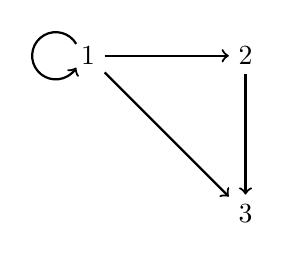
\begin{tikzpicture}
	\node (atom1) at (0,2) {1};
	\node (atom2) at (2,2) {2};
	\node (atom3) at (2,0) {3};
	\draw[->, thick] (atom1)--(atom2);
	\draw[->, thick] (atom1)--(atom3);
	\draw[->, thick] (atom1)+(-0.15,0.15) arc (-330:-30:.3);
	\draw[->, thick] (atom2) -- (atom3);
\end{tikzpicture}
\end{arialabel}
\end{center}

采用 \cref{s:Interpretations} 中使用的约定，这一解释的论域是前三个正整数，并且当且仅当在我们的图中有从 x 指向 y 的箭头时，“$\atom{R}{x,y}$” 对 x 和 y 为真。以下是该解释使其为真的一些语句：

\begin{itemize}
	\item “$\forall x \exists y\, \atom{R}{y,x}$”
	\item “$\exists x \forall y\, \atom{R}{x,y}$” \hfill ($x$ 的见证：$1$)
	\item “$\exists x \forall y (\atom{R}{y,x} \eiff x = y)$” \hfill ($x$ 的见证：$1$)
	\item “$\exists x \exists y \exists z ((\enot y = z \eand \atom{R}{x,y}) \eand \atom{R}{z,x})$” \hfill ($x$ 的见证：$2$)
	\item “$\exists x \forall y\, \enot \atom{R}{x,y}$” \hfill ($x$ 的见证：$3$)
	\item “$\exists x (\exists y\, \atom{R}{y,x} \eand \enot \exists y\, \atom{R}{x,y})$” \hfill ($x$ 的见证：$3$)
\end{itemize}

这立即表明，前面六个语句都是共同可满足的。我们可以利用这一观察来构造\emph{无效}论证，例如：
\begin{align*}
	\forall x \exists y\, \atom{R}{y,x}, \exists x \forall y\, \atom{R}{x,y}  &\therefore  \forall x \exists y\, \atom{R}{x,y}\\
	\exists x \forall y\, \atom{R}{x,y}, \exists x \forall y \enot \atom{R}{x,y} & \therefore \enot \exists x \exists y \exists z (\enot y = z \eand (\atom{R}{x,y} \eand \atom{R}{z,x}))
\end{align*}
以及除此之外的许多其他例子。

\factoidbox{
	如果某个解释使得 $\metav{A}_1, \metav{A}_2, \ldots, \metav{A}_n$ 全部为真而 $\metav{C}$ 为假，那么：


\begin{compactlist}
		\item$\metav{A}_1, \metav{A}_2, \ldots, \metav{A}_n \therefore \metav{C}$ 是\emph{无效的}；并且
	\item $\metav{A}_1, \metav{A}_2, \ldots, \metav{A}_n \nentails \metav{C}$；并且
	\item
	并且 $\metav{A}_1, \metav{A}_2, \ldots, \metav{A}_n, \enot \metav{C}$ 是共同可满足的。
\end{compactlist}
}
能够反驳某个说法（例如对逻辑真理的声称，或对蕴涵的声称）的解释，被称为\emph{反解释（counter-interpretation）}，或称\emph{反模型（counter-model）}。

不过，在结束本节之前，我们要提醒一下（无）有效性与（非）蕴涵之间的关系。回想一下一阶逻辑的局限性：它是一种外延性语言；它忽略了模糊性问题；它无法处理因“特殊原因”而有效的情况。为了展示这些问题中的一个例子，考虑下面这个自然语言论证：

\begin{earg}
	\item[] 每只狐狸都很可爱。
	\item[\texttherefore] 所有雌狐都很可爱。
\end{earg}

这在概念上是有效的：雌狐必然是狐狸，所以前提为真而结论为假是不可能的。那么，我们可以合理地将这个论证符号化如下：
$$\forall x(\atom{F}{x} \eif \atom{C}{x}) \therefore \forall x(\atom{V}{x} \eif  \atom{C}{x})$$
然而，很容易找到反模型来表明 $\forall x(\atom{F}{x} \eif \atom{C}{x}) \nentails \forall x(\atom{V}{x} \eif  \atom{C}{x})$。（\emph{练习}：找一个。）因此，仅仅因为相关的\emph{一阶逻辑蕴涵}存在反模型，就推论出那个自然语言论证是\emph{无效的}，将是\emph{错误的}。

总体的教训是：如果你想要从一阶逻辑中没有某个蕴涵关系，推论出某个自然语言论证是无效的，那么你需要论证，在你的符号化方式中，没有丢失任何重要的东西。

\practiceproblems

\solutions
\problempart
\label{pr.Contingent}
证明以下每一个语句既非有效式也非矛盾式：

\begin{compactlist}
\item \leftsolutions\ $\atom{D}{a}  \eand \atom{D}{b}$
\item \leftsolutions\ $\exists x\, \atom{T}{x,h}$
\item \leftsolutions\ $\atom{P}{m}  \eand \enot\forall x\, \atom{P}{x}$
\item $\forall z \atom{J}{z} \eiff \exists y\, \atom{J}{y}$
\item $\forall x (\atom{W}{x,m,n} \eor \exists y\,\atom{L}{x,y})$
\item $\exists x (\atom{G}{x} \eif \forall y\, \atom{M}{y})$
\item $\exists x (x = h \eand x = i)$
\end{compactlist}

\solutions
\problempart
\label{pr.NotEquiv}
证明以下语句对不是逻辑等价的。

\begin{compactlist}
\item $\atom{J}{a} $,  $\atom{K}{a}$
\item $\exists x\, \atom{J}{x}$,  $\atom{J}{m}$
\item $\forall x\, \atom{R}{x,x}$, $\exists x\, \atom{R}{x,x}$
\item $\exists x\, \atom{P}{x} \eif \atom{Q}{c}$, $\exists x (\atom{P}{x} \eif \atom{Q}{c})$
\item $\forall x(\atom{P}{x} \eif \enot \atom{Q}{x})$, $\exists x(\atom{P}{x} \eand \enot \atom{Q}{x})$
\item $\exists x(\atom{P}{x} \eand \atom{Q}{x})$, $\exists x(\atom{P}{x} \eif \atom{Q}{x})$
\item $\forall x(\atom{P}{x}\eif \atom{Q}{x})$, $\forall x(\atom{P}{x} \eand \atom{Q}{x})$
\item $\forall x\exists y\, \atom{R}{x,y}$, $\exists x\forall y\, \atom{R}{x,y}$
\item $\forall x\exists y\, \atom{R}{x,y}$, $\forall x\exists y\, \atom{R}{y,x}$
\end{compactlist}

\problempart
证明以下语句是共同可满足的：

\begin{compactlist}
\item  $\atom{M}{a}, \enot \atom{N}{a}, \atom{P}{a}, \enot \atom{Q}{a}$
\item $\atom{L}{e,e}, \atom{L}{e,g}, \enot \atom{L}{g,e}, \enot \atom{L}{g,g}$
\item $\enot (\atom{M}{a} \eand \exists x\, \atom{A}{x}), \atom{M}{a} \eor \atom{F}{a}, \forall x(\atom{F}{x} \eif \atom{A}{x})$
\item $\atom{M}{a} \eor \atom{M}{b}, \atom{M}{a} \eif \forall x \enot \atom{M}{x}$
\item $\forall y\, \atom{G}{y}, \forall x (\atom{G}{x} \eif \atom{H}{x}), \exists y \enot \atom{I}{y}$
\item $\exists x(\atom{B}{x} \eor \atom{A}{x}), \forall x \enot \atom{C}{x}, \forall x\bigl[(\atom{A}{x} \eand \atom{B}{x}) \eif \atom{C}{x}\bigr]$
\item $\exists x\, \atom{X}{x}, \exists x\, \atom{Y}{x}, \forall x(\atom{X}{x} \eiff \enot \atom{Y}{x})$
\item $\forall x(\atom{P}{x} \eor \atom{Q}{x}), \exists x\enot(\atom{Q}{x} \eand \atom{P}{x})$
\item $\exists z(\atom{N}{z} \eand \atom{O}{z,z}), \forall x\forall y(\atom{O}{x,y} \eif \atom{O}{y,x})$
\item $\enot \exists x \forall y\, \atom{R}{x,y}, \forall x \exists y\, \atom{R}{x,y}$
\item $\enot \atom{R}{a,a}$, $\forall x (x=a \eor \atom{R}{x,a})$
\item $\forall x\forall y\forall z[(x=y \eor y=z )\eor x=z]$, $\exists x\exists y\ \enot x= y$
\item $\exists x\exists y((\atom{Z}{x} \eand \atom{Z}{y} )\eand x=y)$, $\enot \atom{Z}{d}$, $d=e$
\end{compactlist}

\problempart
证明以下论证是无效的：

\begin{compactlist}
\item $\forall x(\atom{A}{x} \eif \atom{B}{x}) \therefore \exists x\, \atom{B}{x}$
\item $\forall x(\atom{R}{x} \eif \atom{D}{x}), \forall x(\atom{R}{x} \eif \atom{F}{x}) \therefore \exists x(\atom{D}{x} \eand \atom{F}{x})$
\item $\exists x(\atom{P}{x}\eif \atom{Q}{x}) \therefore \exists x\, \atom{P}{x}$
\item $\atom{N}{a} \eand \atom{N}{b} \eand \atom{N}{c} \therefore \forall x\, \atom{N}{x}$
\item $\atom{R}{d,e}, \exists x\, \atom{R}{x,d} \therefore \atom{R}{e,d}$
\item $\exists x(\atom{E}{x} \eand \atom{F}{x}), \exists x\, \atom{F}{x} \eif \exists x\, \atom{G}{x} \therefore \exists x(\atom{E}{x} \eand \atom{G}{x})$
\item $\forall x\, \atom{O}{x,c}, \forall x\, \atom{O}{c,x} \therefore \forall x\, \atom{O}{x,x}$
\item $\exists x(\atom{J}{x} \eand \atom{K}{x}), \exists x \enot \atom{K}{x}, \exists x \enot \atom{J}{x} \therefore \exists x(\enot \atom{J}{x} \eand \enot \atom{K}{x})$
\item $\atom{L}{a,b} \eif \forall x\, \atom{L}{x,b}, \exists x\, \atom{L}{x,b} \therefore \atom{L}{b,b}$
\item $\forall x(\atom{D}{x} \eif \exists y\, \atom{T}{y,x}) \therefore \exists y \exists z\ \enot y= z$
\end{compactlist}

\chapter{关于解释的推理}

\section{有效式与矛盾式}
我们可以通过提供一个精心指定的、使该语句为假的解释，来证明一个语句\emph{不}是有效式。另一方面，要证明某个语句\emph{是}有效式，即使构造出十个、一百个，甚至一千个该语句为真的解释也远远不够。一个语句只有在\emph{每一个}解释下都为真时才是有效式，而解释有无穷多个。我们需要对\emph{所有}解释进行推理，而逐个处理它们是无法实现的！

有时，我们可以相当容易地对所有解释进行推理。例如，我们可以给出一个相对简单的论证来说明 “$\atom{R}{a,a}\eor\enot \atom{R}{a,a}$” 是一个有效式：


\begin{quote}
		\label{allmodels1}
		任何相关的解释都会给 “$\atom{R}{a,a}$” 指派一个真值。如果在某个解释下 “$\atom{R}{a,a}$” 为真，那么在该解释下 “$\atom{R}{a,a} \eor \enot\atom{R}{a,a}$” 为真。如果在某个解释下 “$\atom{R}{a,a}$” 为假，那么 $\enot\atom{R}{a,a}$ 为真，因此在该解释下 “$\atom{R}{a,a} \eor\enot \atom{R}{a,a}$” 为真。只有这两种可能。所以 “$\atom{R}{a,a} \eor\enot \atom{R}{a,a}$” 在每个解释下都为真。因此，它是一个有效式。
	\end{quote}


这个论证当然是有效的，并且其结论为真。然而，它并非一阶逻辑内部的论证。相反，它是用自然语言\emph{关于}一阶逻辑的论证：它是一个元语言中的论证。

另一点值得注意的是，由于所讨论的语句不包含量词，我们无须考虑如何解释 “$a$” 和 “$R$”；关键在于，无论我们如何解释它们，“$\atom{R}{a,a}$” 都会有一个真值。（对于真值函项逻辑的语句，我们最终也可以给出完全相同的论证。）

再举一个例子。语句 “$\forall x(\atom{R}{x,x}\eor\enot \atom{R}{x,x})$” 显然应该是一个有效式。然而，要\emph{精确地}说明原因却颇为棘手。我们不能说 “$\atom{R}{x,x} \eor\enot \atom{R}{x,x}$” 在每个解释下都为真，因为 “$\atom{R}{x,x} \eor\enot \atom{R}{x,x}$” 甚至不是一阶逻辑的一个\emph{语句}（记住 “$x$” 是变元，不是名称）。相反，我们应该这样说：


\begin{quote}
		考虑某个任意的解释。“$\forall x(\atom{R}{x,x}\eor \enot\atom{R}{x,x})$” 在我们的解释中为真，当且仅当 “$\atom{R}{x,x}\eor\enot\atom{R}{x,x}$” 被其论域中的每一个对象所满足。考虑论域中某个任意的成员，为方便起见，我们称之为弗雷迪（Fred）。弗雷迪要么满足 “$\atom{R}{x,x}$”，要么不满足。如果弗雷迪满足 “$\atom{R}{x,x}$”，那么他也满足 “$\atom{R}{x,x} \eor \enot \atom{R}{x,x}$”。如果弗雷迪不满足 “$\atom{R}{x,x}$”，\emph{则}他满足 “$\enot\atom{R}{x,x}$”，因此也满足 “$\atom{R}{x,x} \eor\enot \atom{R}{x,x}$”。\footnote{我们在此利用了联结词的真值条件也适用于满足关系这一事实：$a$ 满足 $\metav{A}(\metav{x}) \lor \metav{B}(\metav{x})$ 当且仅当 $a$ 满足 $\metav{A}(\metav{x})$ 或 $\metav{B}(\metav{x})$，等等。} 所以无论哪种情况，弗雷迪都满足 “$\atom{R}{x,x} \eor\enot \atom{R}{x,x}$”。既然弗雷迪并没有什么特殊之处——我们本可选择任意对象——可见论域中的每一个对象都满足 “$\atom{R}{x,x} \eor\enot \atom{R}{x,x}$”。所以 “$\forall x (\atom{R}{x,x} \eor\enot \atom{R}{x,x})$” 在我们的解释中为真。但我们的解释是任意选取的，因此 “$\forall x (\atom{R}{x,x} \eor\enot \atom{R}{x,x})$” 在每一个解释下都为真。它因此是一个有效式。
	\end{quote}


这番论证相当冗长，但就目前而言，别无他法。为了证明一个语句是有效式，我们必须对\emph{所有}解释进行推理。

\section{其他情况}
类似的观点也适用于其他情况。因此，如果我们想要证明以下情形，就必须对所有解释进行推理：


\begin{itemize}
		\item 一个语句是矛盾式（这要求它在\emph{每一个}解释下为假）；
		\item 两个语句是逻辑等价的（这要求它们在\emph{每一个}解释下真值相同）；
		\item 一些语句是共同不可满足的（这要求不存在一个解释使得所有这些语句同时为真，换言之，在\emph{每一个}解释中，这些语句里至少有一个为假）；
		\item 一个论证是有效的（这要求在前提为真的\emph{每一个}解释下，结论也为真）；
		\item 一些语句蕴涵另一个语句。
	\end{itemize}


问题在于，凭借目前掌握的工具，对所有解释进行推理是极为困难的！看最后一个例子，这是一个再明显不过的蕴涵关系：
	$$\forall x(\atom{H}{x} \eand \atom{J}{x}) \entails \forall x\, \atom{H}{x}$$
毕竟，如果所有东西都既是 $H$ 又是 $J$，那么所有东西都是~$H$。
但我们只能通过考察前提 $\forall
x(\atom{H}{x} \eand \atom{J}{x})$ 为真的每一个解释中什么必须为真，来确立这个蕴涵关系。为此，我们将不得不进行如下推理：

\begin{quote}
	考虑任意一个使“$\forall x(\atom{H}{x} \eand \atom{J}{x})$”为真的解释。由此可知，在此解释中每个对象都满足“$\atom{H}{x} \eand \atom{J}{x}$”。那么，“$\atom{H}{x}$”也将被每个对象满足。\footnote{这里我们再次用到了以下事实：任何满足 $\metav{A}(\metav{x}) \land \metav{B}(\metav{x})$ 的对象都必定同时满足 $\metav{A}(\metav{x})$ 和 $\metav{B}(\metav{x})$。}因此，在此解释中“$\forall x\, \atom{H}{x}$”必定为真。我们除了假定该解释使“$\forall x(\atom{H}{x} \eand \atom{J}{x})$”为真外，并未对其作任何其他假定。所以，任何使“$\forall x(\atom{H}{x} \eand \atom{J}{x})$”为真的解释，也都使“$\forall x\, \atom{H}{x}$”为真。
\end{quote}

即便是这样一个简单的蕴涵，其推理也略显复杂。对于更复杂的蕴涵，推理过程可能会变得极其繁复。

下表总结了对于不同逻辑概念，是单个解释（或反解释）即足以判定，还是必须考虑所有解释。

\begin{center}\small
\begin{tabular}{l l l}
%\cline{2-3}
 & \textbf{是} & \textbf{否}\\
 \hline
%\cline{2-3}
有效性？ & 所有解释 & 一个反解释\\
矛盾式？ & 所有解释 & 一个反解释\\
等价？ & 所有解释 & 一个反解释\\
可满足？ & 一个解释 & 所有解释\\
有效？ & 所有解释 & 一个反解释\\
蕴涵？ & 所有解释 & 一个反解释\\
\end{tabular}
\end{center}

\label{table.ModelOrArgument}

你可以将此表与 \cref{s:PartialTruthTable} 末尾的表格进行比较。关键区别在于，真值函项逻辑处理的是真值表，而一阶逻辑处理的是解释。这一区别至关重要，因为每个真值表都只有有限多行，故而完整的真值表是一个相对容易处理的对象。相比之下，对于任意给定的语句（集），都存在无穷多个解释，因此对所有解释进行推理可能极为棘手。

\chapter{关系的性质}\label{ch:PropRelations}

符号化约定使我们能将二元谓词符号（如“$\atom{R}{x,y}$”）指派给带有两个空位的自然语言谓词，例如“\gap{x} 比 \gap{y} 年长”。这使我们能够将如下论证符号化：

\begin{earg}
	\item Rudolf 比 Kurt 年长。
	\item Kurt 比 Julia 年长。
	\item[\texttherefore] Rudolf 比 Julia 年长。
\end{earg}

该论证是有效的，但其在一阶逻辑中的符号化形式，

\begin{earg}
	\item $\atom{R}{r,k}$
	\item $\atom{R}{k,j}$
	\item[\texttherefore] $\atom{R}{r,j}$
\end{earg}

却并非有效。这是因为该论证的有效性依赖于“$x$ 比 $y$ 年长”这一关系的某个性质，即：如果某人 $x$ 比某人 $y$ 年长，并且 $y$ 也比 $z$ 年长，那么 $x$ 必定比 $z$ 年长。“年长于”这一性质被称为\define{传递性}。我们可以在一阶逻辑中将这一性质\emph{本身}符号化为：
\[
	\forall x\forall y\forall z((\atom{R}{x,y} \eand \atom{R}{y,z}) \eif
	\atom{R}{x,z})
\]
当一个论证的有效性\emph{仅仅}依赖于所涉关系的某个性质，并且该性质可在一阶逻辑中被符号化时，我们可将此符号化形式加入论证，从而得到一个在一阶逻辑中确实有效的论证：

\begin{earg}
	\item $\forall x\forall y\forall z((\atom{R}{x,y} \eand \atom{R}{y,z}) \eif
	\atom{R}{x,z})$
	\item $\atom{R}{r,k}$
	\item $\atom{R}{k,j}$
	\item[\texttherefore] $\atom{R}{r,j}$
\end{earg}

诸如传递性这类关系性质是非常重要的概念，尤其是在逻辑的科学应用中。例如，数字间的序关系（如 $<$ 和 $\le$，以及 $>$ 和 $\ge$）都是传递的。恒等关系 $=$ 也是传递的。

还有其他一些关系性质也因其重要性而拥有名称，并常出现于应用中。以下列举若干：

\factoidbox{
	\begin{factoiditems}
		\item 关系 $R$ 是\define{传递的} \ifeff{} 只要 $\atom{R}{x,y}$ 和 $\atom{R}{y,z}$ 成立，则 $\atom{R}{x,z}$ 也成立。
		\item 关系 $R$ 是\define{自反的} \ifeff{} 对任意 $x$，$\atom{R}{x,x}$ 成立。
		\item 关系 $R$ 是\define{对称的} \ifeff{} 只要 $\atom{R}{x,y}$ 成立，则 $\atom{R}{y,x}$ 也成立。
		\item 关系 $R$ 是\define{反对称的} \ifeff{} 不存在两个\emph{不同的} $x$ 和 $y$，使得 $\atom{R}{x,y}$ 和 $\atom{R}{y,x}$ 同时成立。
	\end{factoiditems}

}

\newglossaryentry{transitive}
{
  name=传递性,
  text = 传递的,
  description={一个关系~$R$具有的性质，当且仅当只要 $\atom{R}{x,y}$ 且 $\atom{R}{y,z}$ 成立，则~$\atom{R}{x,z}$ 也成立}
}
\newglossaryentry{reflexive}
{
  name=自反性,
  text = 自反的,
  description={一个关系~$R$具有的性质，当且仅当对任意~$x$，$\atom{R}{x,x}$ 都成立}
}
\newglossaryentry{symmetric}
{
  name=对称性,
  text = 对称的,
  description={一个关系~$R$具有的性质，当且仅当只要 $\atom{R}{x,y}$ 成立，则 $\atom{R}{y,x}$ 也成立}
}
\newglossaryentry{anti-symmetric}
{
  name=反对称性,
  text = 反对称的,
  description={一个关系~$R$具有的性质，当且仅当找不到两个\emph{不同的} $x$ 和 $y$ 使得 $\atom{R}{x,y}$ 和 $\atom{R}{y,x}$ 同时成立}
}

我们已经看到传递性可以在一阶逻辑中被符号化。其他几项性质也可以：

\begin{itemize}
	\item $R$是自反的： $\forall x\,\atom{R}{x,x}$
	\item $R$是对称的： \[\forall x\forall y(\atom{R}{x,y} \eif \atom{R}{y,x})\]
	\item $R$是反对称的： \[\lnot\exists x\exists y((\atom{R}{x,y}
	\eand \atom{R}{y,x}) \eand \enot x=y)\]或者等价地， \[\forall x\forall y((\atom{R}{x,y}
	\eand \atom{R}{y,x}) \eif x=y)\]
\end{itemize}

表达在某些方面对等的关系是自反的，例如“和……年龄相同”、“和……一样高”，以及其中最严格的等价关系——同一性（等号）$=$。它们也是对称的：例如，当 $x$ 和 $y$ 一样高时，$y$ 也和 $x$ 一样高。事实上，同时具有自反性、对称性和传递性的关系被称为 \define{等价关系}。

等价关系并非唯一的对称关系。例如，“是……的兄弟姐妹”是对称的，但它不是自反的（因为没有人是自己的兄弟姐妹）。

同时具有自反性、传递性和反对称性的关系被称为 \define{偏序}。例如，$\le$ 和 $\ge$ 都是偏序。相比之下，“不比……年长”这个关系是自反且传递的，但不是反对称的。（两个不同的人可能同岁，因此谁也不比谁年长。）

\practiceproblems

\problempart
请举例说明具有下列性质的关系：

\begin{compactlist}
	\item 自反但不具有对称性
	\item 对称但不具有传递性
	\item 具有传递性和对称性，但不具有自反性
\end{compactlist}

\problempart
请通过给出一个使以下两个句子都为真的解释，来证明一个关系可以同时既是对称的又是反对称的：
\begin{align*}
	& \forall x\forall y(\atom{R}{x,y} \eif \atom{R}{y,x})\\
	& \forall x\forall y((\atom{R}{x,y} \eand \atom{R}{y,x}) \eif x=y)
\end{align*}
